\documentclass{standalone}

\usepackage{tikz}
\usetikzlibrary{positioning}
\usetikzlibrary{er}

%% Grid spacing
\newdimen\ERspacing
\ERspacing=3cm

\begin{document}
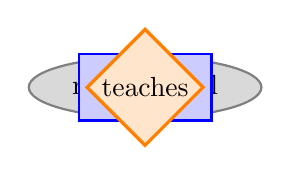
\begin{tikzpicture}
    [
    node distance=\ERspacing and \ERspacing,
    on grid,
    every entity/.style={fill=blue!20, draw=blue, thick},
    every relationship/.style={fill=orange!20, draw=orange, very thick},
    every attribute/.style={fill=gray!30, draw=gray, thick},
    ]

    \node[entity] (ent_scholar)
    {Scholar}
    child {node [key attribute, above left = of ent_scholar] {id}}
    child {node [attribute, above right = of ent_scholar] {name, email}};
    
    \node[relationship, below = of ent_scholar] (rel_is)
    {is}
    edge (ent_scholar)
    child {node [entity, below = of rel_is] (ent_student) {Student}}
    child {node [entity, below right = of rel_is] (ent_admin) {Admin}}
    child {node [entity, below left = of rel_is] (ent_professor) {Professor}};

    \node[relationship, below = of ent_student] (rel_enrolls)
    {enrolls}
    edge (ent_student)
    child {node [entity, below = of rel_enrolls] (ent_class) {Class} child {node [key attribute, right = of ent_class] {id}}};

    \node[relationship, below = of ent_professor] (rel_teaches)
    {teaches}
    edge (ent_professor)
    edge (ent_class);
\end{tikzpicture}
\end{document}
